\subsection{Estimote}
\label{sec:indoor-positioning:estimote}
\todo[author=Thalley]{Skal vi have noget med omkring iBeacon protokollen?}
We choose to use the solution provided by Estimote for this project.
The choice of Estimote was made due to it being available already, 
having a low price which may fit consumers, 
and its advertised ease of use. 
However, as described below the ease of use come at a cost of the accuracy.
Furthermore Estimote has put effort into optimizing their software for indoor positioning, 
and has released a software development kit (SDK),
that developers can use to perform indoor positioning, 
making it easier to adopt the technology.

Estimote, aside from offering the typical use case for beacons like entering a specific region, 
has also specialized in indoor location of users using the iBeacon protocol. 
The company has developed and released the Estimote Indoor Location SDK\footnote{https://github.com/Estimote/iOS-Indoor-SDK}.
They have also released a demo application for iOS\footnote{https://itunes.apple.com/us/app/estimote-indoor-location/id963704810}, 
which is meant to ease configuration needed for indoor location. 

A user will install the beacons in a room by placing a minimum of \num{4} beacons on the walls, 
preferably in the middle of each wall in a rectangular room.   
Next the user walks along the perimeter of the room, 
and thereby registering the location of the beacons, 
by collecting signal strengths from the beacons (a feature of the iBeacon protocol), 
and data from the phones accelerometer and/or gyroscope.
After the configuration, the application will have estimated the length of and placement of the walls, 
along with the signal strengths of each beacon.

To analyze the precision, 
to see whether we could actually use these beacons and Estimote's SDK, 
we performed a few tests. 
During our tests we found that the approach for configuring the indoor positioning, 
as described above, works terribly or not at all. 
After configuring the room, 
the application would show an illustration of the registered room, 
and we found the measurements to to be very inaccurate.
We have decided not to use the built-in room configuration. 
\todo[author=Thalley]{Indsæt nogle beskrivende tal eller illustrationer til at forklare hvor ringe det faktisk var}

\subsubsection{Configuring Rooms Programmatically}
As mentioned, Estimote provides the Estimote Indoor Location SDK, 
for performing indoor positioning using beacons on iOS. 
The SDK provides two mechanisms for configuring a room for indoor positioning.

\begin{enumerate}
\item Using the built-in controller. The component presents the user with a guided configuration similar to the one used in the Estimote Indoor Location application.
\item Programmatically using the \texttt{ESTLocationBuilder} class.
\end{enumerate}

The built-in controller was abandoned as it resulted in poor accuracy.

The \texttt{ESTLocationBuilder} lets developers configure a room programmatically, 
by passing coordinates (\texttt{ESTPoint}s) and an orientation to the builder. 
The $X$ and $Y$ value of each coordinate is measured in meters. 
Therefore a set of coordinates $\{(0, 0$), $(0, 5)\}$ represents a horizontal line of $5$ meters, 
and the set of coordinates $\{(0,0),(0,5),(5,5),(5,0)\}$ represents $5$ by $5$ meter room.

\begin{listing}
\begin{swiftcode}
        let locationBuilder = ESTLocationBuilder()
        locationBuilder.setLocationBoundaryPoints([
            ESTPoint(x: 0.cmToMeter(), y: 0.cmToMeter()),
            ESTPoint(x: 537.cmToMeter(), y: 0.cmToMeter()),
            ESTPoint(x: 537.cmToMeter(), y: 60.cmToMeter()),
            ESTPoint(x: 690.cmToMeter(), y: 60.cmToMeter()),
            ESTPoint(x: 690.cmToMeter(), y: 385.cmToMeter()),
            ESTPoint(x: 0.cmToMeter(), y: 385.cmToMeter()),
        ])
        
        let ice3 = "dec18deac0c5"
        let blueberry3 = "f13173ad3185"
        let ice2 = "d470d26d33f3"
        let mint3 = "e6d39dee79c9"
        
        locationBuilder.addBeaconIdentifiedByMac(blueberry3, atBoundarySegmentIndex: 0, inDistance: 422.cmToMeter(), fromSide: .RightSide)
        locationBuilder.addBeaconIdentifiedByMac(ice3, atBoundarySegmentIndex: 3, inDistance: 222.cmToMeter(), fromSide: .RightSide)
        locationBuilder.addBeaconIdentifiedByMac(mint3, atBoundarySegmentIndex: 4, inDistance: 335.cmToMeter(), fromSide: .LeftSide)
        locationBuilder.addBeaconIdentifiedByMac(ice2, atBoundarySegmentIndex: 5, inDistance: 165.cmToMeter(), fromSide: .LeftSide)
        locationBuilder.setLocationOrientation(130)
        locationBuilder.setLocationName("Living Room")
        
        let location = locationBuilder.build()
\end{swiftcode}
\caption{Example usage of the \texttt{ESTLocationBuilder} class.}
\label{lst:estlocationbuilder}
\end{listing}

\Cref{lst:estlocationbuilder} shows how we used the \texttt{ESTLocationBuilder} to create a model of a real world living room. 
The resulting model is illustrated in \Cref{fig:estlocationbuilder-livingroom}.

\begin{figure}[!htb]
  \centering
  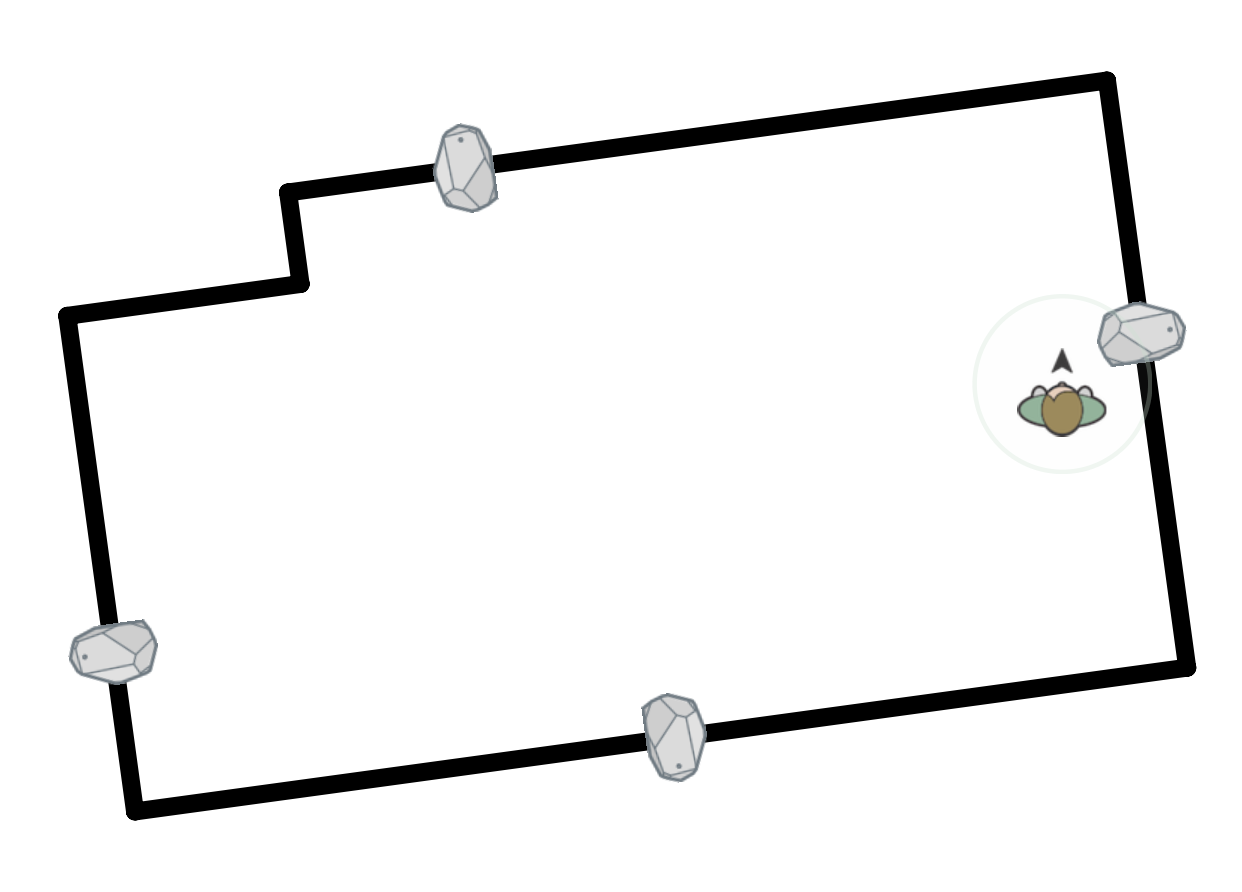
\includegraphics[width=0.33\textwidth]{images/living-room}
  \caption{Model created using the \texttt{ESTLocationBuilder} as shown in C\ref{lst:estlocationbuilder}. Note that the model is rotated accordingly to the orientation of the room and the position of north relative to the user.}
  \label{fig:estlocationbuilder-livingroom}
\end{figure}

The builder is configured with $6$ coordinates that gives information about the shape of the room. 
Next, the beacons are added to the walls of the room. 
Beacons are added with the identifier of the beacon, 
such as \texttt{dec18deac0c5} for the \texttt{ice3} beacon. 
Lastly the orientation of the room relative to north and the name of the room is set. 
When the room has been configured, 
it can be stored on the users Estimote account using the Estimote SDK.
Using the \texttt{ESTLocationBuilder} to model a room reduces any uncertainties in estimating the users location, 
caused by an imprecise model of the room.

\subsubsection{Ranging in the Background}

There are two distinct ways of locating a user when using the iBeacon protocol \cite{estimote:monitoring-ranging}.

\begin{itemize}
\item Region monitoring is performed to check if a user enters or leaves a specific region. A region is a geofence, \ie a virtual perimeter around some location. A region can be used to check if a user arrives or leaves his house, his workplace or if he is nearby a shop encapsulated in a geofence. Regions are useful for performing simple home automation, \eg turn the lights on when the user arrives at home and turn them off when they leave.
\item Ranging is more granular than region monitoring and is used to continuously retrieve the set of beacons in range, along with an estimated distance to them based on the signal strengths. Ranging is used to get a granular user position.
\end{itemize}

According to both Apple and Estimote it is preferred that ranging is only performed while the application is in the foreground, 
\ie the application is on the screen and the user is likely to interact with the application. 
The reason for this is that ranging for beacons can have a negative impact on the battery life, 
whereas the region monitoring does not use as much battery power.

While Apple and Estimote advise against performing beacon ranging in the background, it is possible \cite{apple:monitoring-ibeacon} \cite{estimote:monitoring-ranging}.

%%% Local Variables:
%%% mode: latex
%%% TeX-master: "../../master"
%%% TeX-command-extra-options: "-shell-escape"
%%% End:
